\documentclass[12pt,a4paper]{article}
\usepackage{ucs}
\usepackage{caption}
\usepackage[latin1,utf8x]{inputenc}
\usepackage{amsmath}
\usepackage{caption}
\captionsetup{font=small,labelfont=bf}
\usepackage[danish]{babel}
\usepackage[rmargin=3cm,tmargin=3.3cm]{geometry}
\usepackage{listings}
\setlength{\parindent}{0pt}
\setlength{\parskip}{1ex plus 0.5ex minus 0.2ex}
\usepackage{graphicx}
\usepackage{fixltx2e}

%insert links
\usepackage{hyperref}
\usepackage{fancyhdr,lastpage}	
\pagestyle{fancy}

%header
\lhead{ 
	Embedded Systems \\
	02131 \\ 
}
\chead{ 
}
\rhead{ 2 October, 2012 \\ \bigskip  }

%Footer
\lfoot{
	\rule{\textwidth}{0.1mm}\\
}

\cfoot{}
\rfoot{\ \\ \scriptsize{Side \thepage\ af \pageref{LastPage}}}

\begin{document}

%Forside
\begin{titlepage}
	\begin{center}
		\vspace*{13\baselineskip}
		\huge
		\bfseries
		Embedded Systems\\ 
		\ \\
		02131 \\[5\baselineskip]

		\normalfont
		\Large
		R-peak detection!\\	

		\small
		\vfill
	\end{center}	
	\begin{flushleft}
		Bastian Buch, s113432\\
	 	Jacob Gjerstruo, s113440\\
	\end{flushleft}
\end{titlepage}

\ \\
\section*{Abstract}
The main task of this assignment was to develop the software for a Electro-Cardiogram (ECG) scanner using the Pan-Thompkins QRS-Detection Algorithm. By using this algorithm and writing a program in C we have created a program capable of determining a persons heartbeat from a set of data gathered from a ECG scanner. Our conclusions are that this is entirely feasible, and we recommend the implementation of this algorithm, though it is desirable to make the calculations using hardware, in order to optimize the running speed and make the calculations dynamic.
\thispagestyle{empty} 
\newpage

%Table of Contents
\tableofcontents
\thispagestyle{empty} 
\newpage

%Reset pagecount
\setcounter{page}{1}

%Alm. sider
\ \\
\section{Introduction}
	The company Medembed have hired us to investigate whether the Pan-Thompkins QRS detection algorithm might be used when the company is sending out their next product. This product is a wearable ElectroCardioGram scanner - hereafter just shortened to ECG scanner.\\
	The first task we were given was to implement this algorithm in C, and hereafter, we were tasked with determining whether the algorithm is suited to be implemented in an embedded system.\\
\\
	The algorithm in itself consists of two parts - a filter-part, which consists of 5 different filters, and a detection-part, that consists of various functions for determining whether the input from the ECG-scanner is an R-peak. Once this is done, a program analysis will take place, in which we will analyse the time it takes for the program to run, as well as energy consumption and code size. Furthermore, during this program analysis, we will also discuss our choices, explaining why we have done as we have.\\
\\
\subsection{Requirements}
For this assignment, we initially sat down and looked over the requirements, and in total, we found 5 functional requirements and one non-functional requirement. They are as follow: \\
\\
\textbf{ Functional requirements for the application:}
\begin{itemize}
	\item Correct data acquisition in simulated real-time
	\item Implementation of the 5 filters
	\item Implementation of the RPeakDetection
	\item Correct output of relavant data to the user, based on the algorithm
	\item An analysis of our implementation, including an analysis of the critical parts, runtime and memory requirements.
\end{itemize}
\textbf{Non-functional requirements for the application:}
\begin {itemize}
	\item The programming language used for this is C
\end{itemize}

\section{Analysis}
 	In designing the program for the wearable ECG scanner, there are a few things that needs to be considered:
\begin{enumerate}
	\item How should the real-time data acquisition be simulated?
	\item How should the filters be integrated?
	\item How should the RPeakDetection be integrated?
	\item Which data are relavant for the user, and how should it be shown?
	\item How do you determine the critical parts?
\end{enumerate}

\subsection{Problem 1: Data acquisition in real-time}
	In the product specification for the ECG scanner, we were limited to working with a dataset and not a real patient. To ensure that the product is ready for implementation into a real scanner, one of the requirements is that we do not load the whole dataset into one array, and then work on this one. Instead, we were asked to make sure the data acquisition happens in real time, and this provides a few challenges, the biggest being how to ensure that the program runs through the entire dataset, no matter the size.

\subsection{Problem 2: Integration of Filters}
	In the product specification, we were given 5 filters which all were to be implemented. 4 out of the 5 filters consists of a complicated formula that uses both the current data point, but also previous data points. This creates two issues:
\begin{enumerate}
	\item How should the both the current and the previous data points be transferred from the program to the filters?
	\item How to ensure there's no data under- and overflow?
\end{enumerate}
To the first problem, there were two solutions: Either, one could use a struct or one could use two arrays, one with the data that we operate on and one with data that has already been calculated.\\
To the second problem, the easiest would be to implement the formula with strict if/else sentences, stating specificly when a certain subformula should be used.

\subsection{Problem 3: Integration of RPeakDetection}
After applying all filters to the data it remains to determine what constitutes a heartbeat and how to analyze the hearbeats of the patient. The data acquired from the filters contains peaks, which are analyzed and adapted on the fly to ensure that the patients heartbeats are correctly tracked. All peaks larger than a certain threshold are qualified as heartbeats - referred to as Rpeaks - and data is assembled based on this peak in order to classify further peaks as either heartbeats or noise with as great clarity as possible. This introduces the following issues:
\begin{enumerate}
\item How do we determine whether the patient suffers from irregular and/or weak heartbeasts?
\item How do we ensure that we pick up every heartbeat from the patient?
\end{enumerate}
The problems are solved through the adaption of the criteria for what constitutes a heartbeat. By altering the threshold for Rpeaks depending on the estimated value of a heartbeat, it is possible to dynamically adapt peak detection to the patients heartbeat. If the threshold ends up exceedingly low, we can conclude that the patient has a weak heartbeat, and therefore is in need of medical examination.\\
Furthermore, by establishing the time between each hearbeat, we can deduce the patients heartbeats per minute, which can also help determine if the patient needs examination or not. Finally, if the patients heartbeat strength (deduced from the peaks) differ wildly, the patient has an irregular heartbeat and should also see a doctor immediately.

\subsection{Problem 4: Relavant data}
	To ensure that the patient are given early warnings of a pending heart problem, certain data must be shown to the patient. The requirements themself states that the program must show the value of the latest R-peak detected, the time-value at which it occured and the patients pulse. In addition to those, the requirements also states that the patient should be given a warning if the R-peak value is less than 2000 and if 5 successive RR-intervals has missed the RR-LOW and RR-HIGH values. How these data are shown, however, is not defined.\\
\\
There are various ways to show these data. The first way to do so would be to just make a simple text-based screen where the information would be updated as we calculate them.\\
Alternatively, they could be plotted and a graph over the data could be shown.\\
These two could also be combined, giving both a graph that is updated in real time, as well as text-based information below the graph with the data specified in the requirements.\\
Furthermore, ideally the data and warnings should be displayed in a way easy for the user to understand.

\subsection{Problem 5: Critical parts}
When speaking of critical parts, there are two terms that needs to be discussed - memory requirements and time consumption. This is so because the more memory a program requires, the more physical memory the device must have and therefore, it becomes larger and more power-consuming (in this case, it is the latter that we are interested in). Likewise, as we were given a frequency rate of 250 reads per second, if our functions are very time consuming, we need a strong processor that will be more power-consuming. Therefore, the problem has the following challenges:
\begin{enumerate}
\item What is the estimation of memory usage, and can this be lowered?
\item How fast does the program run, and can it be improved?
\end{enumerate}

\section{Design}
	In designing our program, we very quickly decided to split the program into 4 smaller pieces. Each piece would then consist of functions native to the file - meaning that all filters were placed in the same file, all functions native to the RPeakDetection were placed in the same file, the function that scans the dataset were placed in the same file and they would all be run from a seperate file.\\
\\
	Futhermore, we decided that we would only hold up to 50 data points from the scanner at any given time - we decided that this was the optimal number, as if you went much lower, you risked not having enough data points for some of the filters, and having many more would just be a waste of memory. We also decided to go with 6 arrays with room for 50 data points - one to hold the "raw" data, and five arrays to hold filtered data, one for each filter. This was a nescesity to ensure we had both the x- and the y-values needed in the formula for the filters.\\
\begin{figure}[h!]
  \centering
    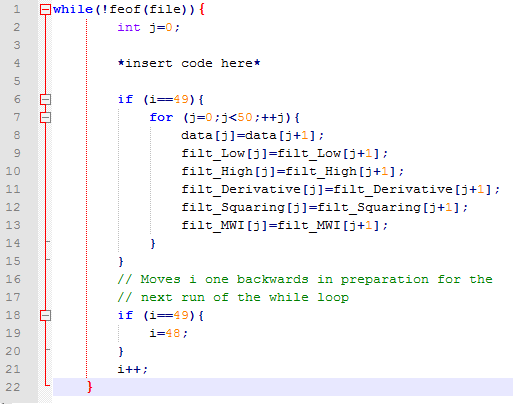
\includegraphics[width=0.8\textwidth]{moveback_loop.png}
  \caption{The code for the for-loop that moves all data points one step backwards, in preperation for the next run}
\end{figure}
\\

\section{Implementation}
\subsection{Solution one: Real-time data acquisition}
As already described, the product specification stated that we needed to do the data acquisition in real time. To solve this, we looked back to the first introductionary exercises we did and used the while-loop we had created back then to run through the dataset. We then ensured that after each data-scan, the data was parsed to each filter and then to RPeakDetection, thus simulating that we received each data point one at a time, coinciding with each run through the filters with the while loop. The most important part in this process is, of course, the while loop, that would look something like this:\\
\begin{figure}[h!]
  \centering
    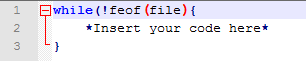
\includegraphics[width=0.5\textwidth]{whileloop.png}
  \caption{The while loop used for real-time data acquisition.}
\end{figure}
\\
The condition in the while loop is simply that as long as fscanf returns true (that is, any other number than 0), it will continue to scan a new number. The fscanf will continue to return true as long as there's a new data point to be scanned, and thus, it will run to the end of the file. Within the body of this while loop would then be the function-call to each of the filters, as well as the function-call to the RPeakDetection. 

\subsection{Solution two: Integration of Filters}
In regards to the first subproblem with the filters, we decided to solve the problems with the integration of the filters by using two arrays - one that holds the raw data that we needed to operate on, and one that holds the data that had already been filtered. We then used these arrays as input parameters, as well as an integer that holds the position in the array that we are currently operating on.\\
In regards to the second, we decided to take the natural approach and implement each filter with if/else sentences, thus ensuring that we would not move beyond the lower bounds of the two input-arrays with data. Each formula were split up according to the various x\textsubscript{n-z} where x is the array, n is the position we are operating on and z is an integer specified by the formula. Below is an example of this - it is our lowpass-filter, where each if-statement refers to a specific part of the formula.\\
\begin{figure}[h!]
  \centering
    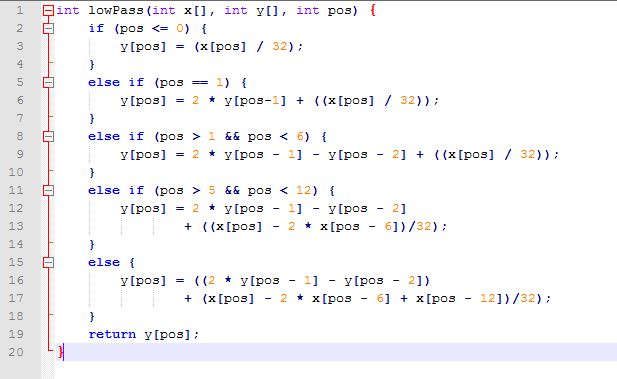
\includegraphics[width=0.75\textwidth]{filter_example.png}
  \caption{An example of the implementation of one of the filters.}
\end{figure}
\subsection{Solution three: Integration of RPeakDetection}
We implemented the detection by sorting our recieved data into an array consisting entirely of peaks. These peaks were then tested against our threshold for what constitued a peak. These values would change upon sucessfully finding a peak, dynamically altering the requirements for what constitutes a heartbeat. After confirming a heartbeat, the time between each heartbeat would be deduced through the "time" between each heartbeat in samples, knowing that for every 250 samples, a second has passed. Although the filters introduce a delay in the data treatment, this delay is applied to all heartbeats and therefore has no bearing on the heartbeats per minute, which can finally be deduced by scaling our results to 60 seconds. By creating and dynamically altering an average of the latest eight heartbeats, we could also determine when a heartbeat was "due" and thus determine if the heartbeats are irregular, if they appear too late or too early. Should no heartbeat appear, a search through all previous beats takes place to a reduced threshold, under the assumption that the heartbeat took place, but was simply too weak to be noticed by the initial threshold. The variables are dynamically altered in every case where a beat is found, thereby increasing the chance no further beats are missed.
\subsection{Solution four: Relavant data}
Due to time constraints, we decided to just go with a text-based screen that would show the required data and warnings in the initial version of the program. This was accomplished by a few simple print statements - however, in the finished product, we would implement the combined solution - giving the user both a graph (with appropriate markers for the thresholds) as well as a text based menu below with the exact data written out.
\subsection{Solution five: Critical parts}
To analyse the speed, we were given the gprof-tool, which is a profiler that checks the time spent on the entire program, as well as on each function. Figure 4 shows the results given by the profiler run on the main program, which consists of the reading of data from the dataset as well as the 5 filters. Originally, it should've held the function used for determining RPeaks, but due to time constraints, we did not manage to implement this.\\
\begin{figure}[h!]
  \centering
   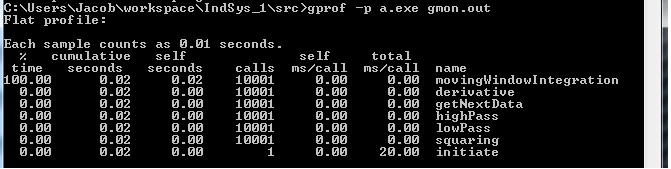
\includegraphics[width=1\textwidth]{results_time.png}
  \caption{The table above shows the time spent in the various filters in our program}
\end{figure}
\\
As can be seen, the 5 filters are each called 10001 times, which is the total number of datas in the dataset we operate on. What's also easily seen is that all the program in itself runs very fast - in fact, making these 50000 function calls takes only around 0.02 seconds, and of all those calls, the main time is spent in the movingWindowIntegration filter - in fact, all other filters takes less than 0.00 seconds, and thus are not even noteworthy of attention at this current time. It should be noted, though, that the current test were run on an intel core I7 with a high clock frequency, primarily used for high-end laptops, and as such, the functions will most likely take much longer time on the final device, as there is absolutely no reason to use such a high-end processor, considering that its power requirements are also quite high - at iddle, the processor uses around 30watt, and at load, it requires between 60 and 90 watt\cite{power consumption}.

\section{Results}
\subsection{Testresults of filters}
Initially, we produced a simple test for the 5 filters. Each of these tests reads in 3000 data points from the a data set, starting out with the initial data given to us, and runs through the filters for these data. The tests then reads another 3000 data points into an array - these data points are found in the files given to us for checking, containing data that has already been run through the filters. We then check the data that we have found by running our filters, with the check-data and the results can be found below:
\begin{figure}[h!]
  \centering
    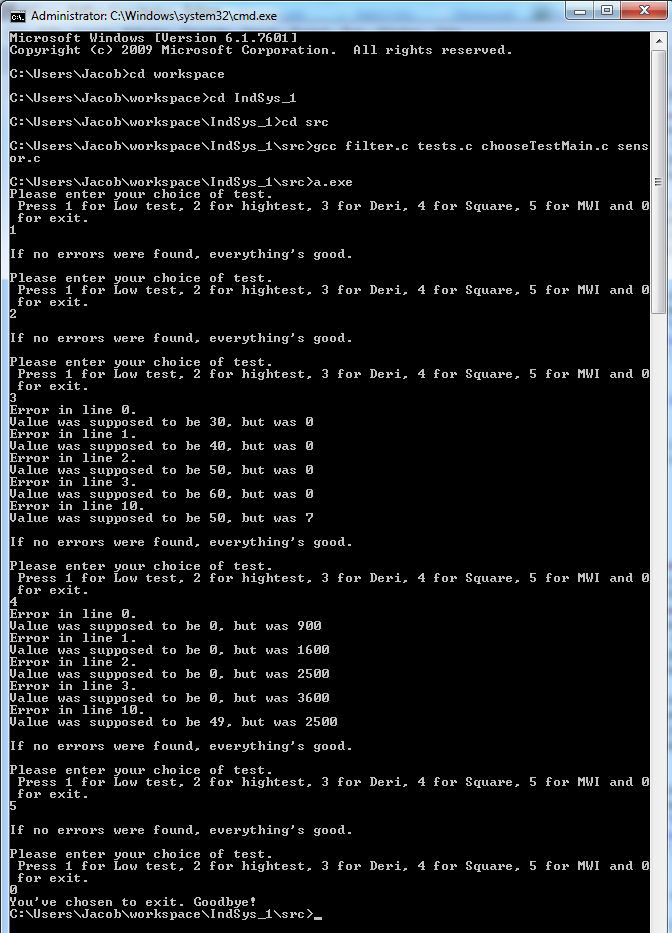
\includegraphics[width=0.5\textwidth]{Results_test.png}
  \caption{The results of our test cases of the 5 filters.}
\end{figure}
\\As can be seen, we also created a small menu for choosing how to navigate these tests, and the Low- and highpass filter, along with the MovingWindowIntegration filter runs without any problems. However, the derivative and the squaring filter reports an error in line 1 through 4, as well as in line 11 (it should here be noted that the program in itself shows line 0 through 3 + 10 - this is because the arrays that are checked start at the position of 0 rather than 1). We estimate that these errors are due to errors in the check-files, as we have manually computed the values for these specific data points and arrive at the same conclussion as our program does, and not as the check files (i.e. 0 for data point 1 through 4 and 7 for data point 11 in the derivative filter, and 900, 1600, 2500, 3600 and 2500 for the values of 1 through 4 and 11 for the squaring filter).
\subsection{Testresults of RPeakDetection}
In order to test our RPeakDetection, we tested a file of 3000 points of data. First, we used a function to determine all peaks and add them to a seperate array, then we ran RPeakDetection on that array.\\
Up untill a certain point, our results correlated with the expected results. After data point 2046, however, we recieved no further peaks. Through testing we have deduced that the error is related to SPKF and the way it interacts with our threshold for what constitutes a peak. Up untill this point, however, everything runs smoothly. 

\section{Discussion}

Through testing of RPeakDetection we have determined our issue is in our Searchback function; after this function is called, our SPKF-value increases extremely, to a point wherein no further heartbeats will cross the threshold. Our results are still accurate, however. 


\section{Conclussion}
We managed to create a program that fulfills the requirements for the filters – these runs and returns the correct value, which has been shown in the tests.
We also created a program that, mostly, did as it was supposed to do in terms of finding R-peaks. This part were tested for the first 3000 data points, too, and did register the r-peaks for the first 2046 data points. However, after this point, something went inexplicedly wrong, and we did not have time to identify what this was. Up to this point, however, it calculates correctly and updates all the variables correctly – both arrays and integers. To be certain these data were saved correctly, we made various print statements during our implementation, both in the main body of the test, as well in the functions themselves, and these showed that the data were saved correctly.
\newpage
\begin{thebibliography}{9}

\bibitem{lamport94}
  Michael Reibel Boesen, Linas Kaminskas, Paul Pop, Karsten Juul Frederiksen\\
  \emph{Assignment 1: Software implementation of a personal ECG scanner}\\
  3rd Edition\\
  2012.

\bibitem{power consumption}
	http://www.notebookcheck.net/typo3temp/pics/afd0f78c47.gif\\
	Date of use: 09/10/2012
\end{thebibliography}
	
\newpage	
	\begin{Large}
		\textbf{Appendix}
	\end{Large}
	\appendix

\section{Who wrote what}
Jacob Gjerstrup, s113440 wrote: Chapter 1, 2 (appart from 2.3), 3, 4 (appart from 4.3), 5.1, 7, appendix\\
Bastian Buch, s113432 wrote: Abstract, chapters: 2.3, 4.3, 5.2, 6.\\
	
\section{Sourcecode - introductionary exercises}
\subsection{ReadFromFile}
	Below is the sourcecode for the introductionary-exercise (From september the 5th) - more precisely, the ReadFromFile source-code.\\
	\\
	\lstinputlisting{ReadFromFile.c}

\subsection{HelloWorld}
	The next is the sourcecode from the same exercise - this time, it's the sourcecode of our HelloWorld program.\\
	\\
	\lstinputlisting{HelloWorld.c}
	
\section{Sourcecode - the real program}
	Below follows the sourcecode for each of the parts of our program, split into sections. The first part, the program, is where the various functions are called, and all our data is stored. The Filter.c contains the 5 different filters. The RPeakDetection contains the detection of each peak, along with the calculations of the various thresholds. The sensor is what scans data from the file, and thus simulates that we scan the patient, and finally, the header files is what contains all the prototypes for our functions.
\subsection{Program}
	\lstinputlisting{program.c}	
\subsection{Filters}
	\lstinputlisting{filter.c}
\subsection{RPeakDetection}
	\lstinputlisting{RPeakDetection.c}	
\subsection{Sensor}
	\lstinputlisting{sensor.c}	
\subsection{Header files}
\subsubsection{sensor.h}
	Below is the first of our headerfiles, called sensor.h. This file contains only the prototype for our sensor.\\
	\lstinputlisting{sensor.h}
\subsubsection{filter.h}
	After this one, the next header file called filter.h comes - this file contains the prototypes of our filters.\\
	\lstinputlisting{filter.h}
\subsubsection{RPeakDetection.h}
	As the last headerfile, we've RPeakDetection.h that contains the prototypes for the functions nescesary for finding an RPeak.
	\lstinputlisting{RPeakDetection.h}
\subsection{Tests}
	We decided to do a run of tests, as discussed in the report. Below is the sourcecode for the tests:
\subsection{Tests of RPeakDetection}
	\lstinputlisting{RPeakTest.c}
\subsubsection{tests}
	\lstinputlisting{tests.c}
\subsubsection{Main function for test cases}
	\lstinputlisting{chooseTestMain.c}
\end{document}